\documentclass{article}

\usepackage{graphicx}
\usepackage{subfigure}
\usepackage[hypcap]{caption}
\usepackage{listings}
\usepackage{float}
\floatstyle{plaintop}
\restylefloat{table}

\title{Experimental Design and Data Analysis: Assignment 6}
\author{Andrew Bedard(2566978) \& Simone van Gompel(2567525) \\ Group 19}

\begin{document}

  \maketitle

  \section*{Exercise 1}
    \subsection*{1}
      The data in \textit{fruitflies.txt} is loaded, and a column: loglongevity, containing the logarithm of the number of days until death can be added to the data by using the R-code found in sec 1.1
      
    \subsection*{2}
      In Fig:\ref{fig:PairFruit} a pairplot of the fruitflies data is seen. It is possibly to discern a relationship between thorax and longevity, and a more linear relationship between thorax and log(longevity).
      Activity and thorax themselfs have no correlation, which is good, because that is part of the experiment set up.
      \begin{figure}[H]
          \centering
          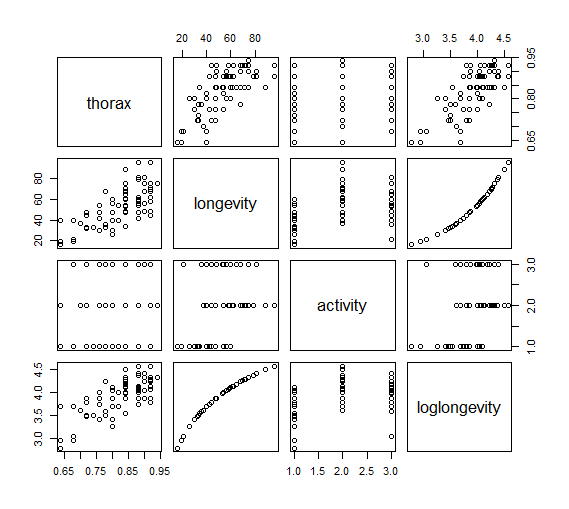
\includegraphics[scale=0.3]{../results/fruitflies2.png}
          \caption{Pairsplot Fruitflies data}
          \label{fig:PairFruit}
      \end{figure}

    \subsection*{3}
      Using ANOVA without taking thorax length into account, we obtain:
            \begin{lstlisting}[language=R]
Response: loglongevity
          Df Sum Sq Mean Sq F value    Pr(>F)    
activity   2 3.6665  1.8333  19.421 1.798e-07 ***
Residuals 72 6.7966  0.0944                      
---
Signif. codes:  
0 ‘***’ 0.001 ‘**’ 0.01 ‘*’ 0.05 ‘.’ 0.1 ‘ ’ 1     
      \end{lstlisting}
      thus with a p-value of $p=1.931e^{-7}$ we reject the null hypothesis that activity does not influence longevity, thus we conclude activity does have an influence on longevity.

    \subsection*{4}
      From the summary of our data on activity and longevity, shown in Table\ref{table:SumAction} we can see a clear trend that as activity increases, the estimated value for longevity decreases.
      \begin{table}[H]
      \begin{center}
      \begin{tabular}{l|lll}
          \hline
                  & isolated& low & high \\
          \hline
          min     & 37      & 21  & 16 \\
          median  & 62      & 56  & 40 \\
          mean    & 63.56   & 56.76 & 38.72  \\
          max     & 75      & 81  & 60 \\
          \hline
      \end{tabular}
      \caption{Summary data of the different actions and longevity}
      \label{table:SumAction}
      \end{center}
      \end{table}
      
      Further if we observe a box plot of the log(longevity) in fig 2 for all three activity levels, we observe a small decrease in longevity from isolated to low, and a dramatic decrease from low to high.
      \begin{figure}[H]
          \centering
          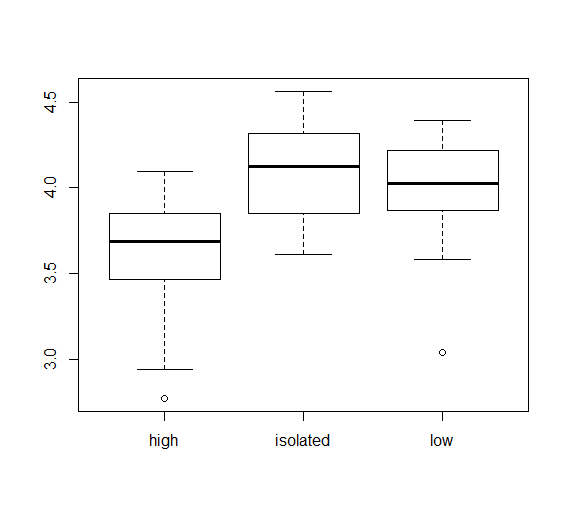
\includegraphics[scale=0.3]{../results/BoxActivity.png}
          \caption{Boxplot of the influence of activity on loglongevity}
          \label{fig:BoxActivity}
      \end{figure}

    \subsection*{5}
    Following the same procedure as exercise 1.3 including thorax length, we obtain the following results using ANOVA:
    \begin{lstlisting}[language=R]
Analysis of Variance Table

Response: loglongevity
          Df Sum Sq Mean Sq F value    Pr(>F)    
activity   2 3.6665  1.8332  44.606 2.838e-13 ***
thorax     1 3.8786  3.8786  94.374 1.139e-14 ***
Residuals 71 2.9180  0.0411                      
---
Signif. codes:  
0 ‘***’ 0.001 ‘**’ 0.01 ‘*’ 0.05 ‘.’ 0.1 ‘ ’ 1       
      \end{lstlisting}
      Again we see that even with thorax length taken into account, with a p-value of $2.838e^{-13}$ we reject the null hypothesis that activity does not effect longevity.

    \subsection*{6}
    From our summary:
        \begin{lstlisting}[language=R]
Coefficients:
                 Estimate Std. Error t value Pr(>|t|)    
(Intercept)       1.21893    0.24865   4.902 5.79e-06 ***
activityisolated  0.40998    0.05839   7.021 1.07e-09 ***
activitylow       0.28570    0.05849   4.885 6.18e-06 ***
thorax            2.97899    0.30665   9.715 1.14e-14 ***
---
Signif. codes:  
0 ‘***’ 0.001 ‘**’ 0.01 ‘*’ 0.05 ‘.’ 0.1 ‘ ’ 1 
      \end{lstlisting}
      We are able to obtain a linear model that will allow us to estimate longevity for various conditions, thus our model is:
      \[
      log(longevity) = 1.219 + 0.4099*(activity isolated) + 0.2857*(activity low) +2.9789*(thorax)
      \]

The mean for thorax length is 0.8245, thus by plugging in values we determine that for mean thorax length our estimates for log(longevity) are:
\begin{itemize}
\item For high activity: 3.6752
\item For low activity: 3.9609
\item For isolated: 4.0852
\end{itemize}

The minimum thorax length is 0.64, so again by plugging in values into our linear model we obtain estimates for log(longevity) for the minimal thorax length of:
\begin{itemize}
\item For high activity: 3.1255
\item For low activity: 3.4112
\item For isolated: 3.5355
\end{itemize}

So it is clear that sexual activity decreases longevity, even for flies with varying thorax length.

    \subsection*{7}
    As we can see in figure 3, thorax length appears to increase longevity, and this holds true for all activity levels.
      \begin{figure}[H]
          \centering
          \subfigure[Thorax length vs log(longevity)]
          {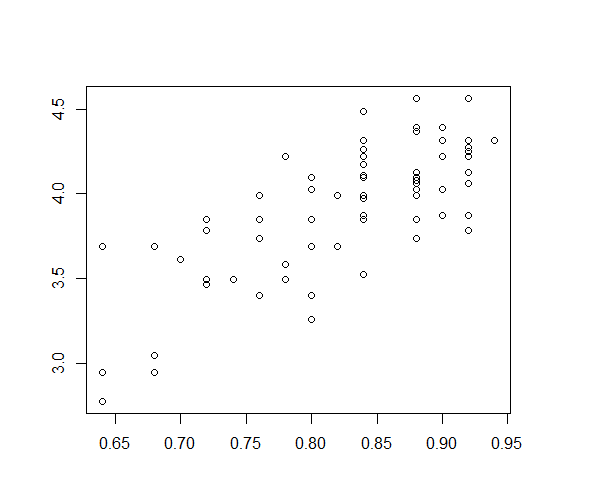
\includegraphics[scale=0.3]{../results/ScatterThorax.png}}
          \subfigure[Thorax length and Activity]
          {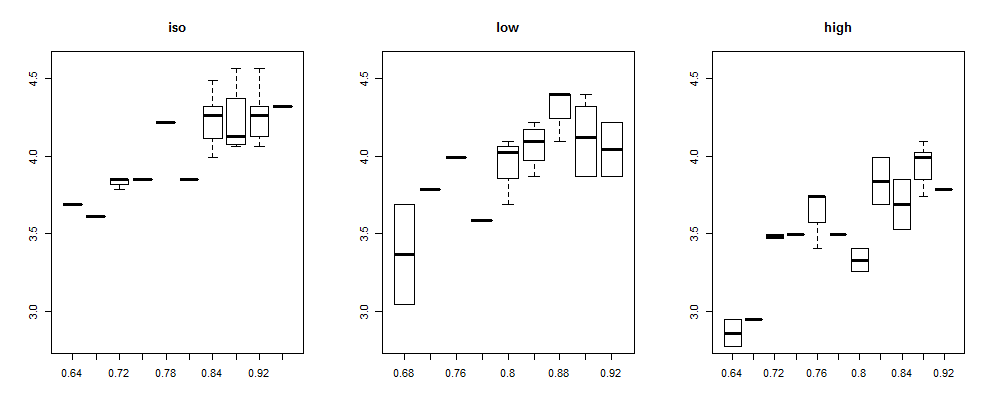
\includegraphics[scale=0.3]{../results/diffThoraxActivity.png}}
          \caption{Boxplot of the influence of thorax length on loglongevity}
          \label{fig:BActivityT}
      \end{figure}

    \subsection*{8}
      Our preference is the analysis without thorax length, this is because the analysis of the data is harder the more variables are included, and according to our research question we are trying to determine the effect of sexual activity on the longevity of fruit flies. Now that we know thorax length increases longevity across all sexual activity levels, we can safely ignore its effects.

    \subsection*{9}
      In Fig\ref{fig:eval} the analysis that includes thorax length is evaluated.
      The qqplot shows that the residuals are normally distributed and the Fitted vs Residuals plot shows that the data has no heteroscedasticity.
      \begin{figure}[H]
          \centering
          \includegraphics[scale=0.3]{../results/evalWithThorax.png}
          \caption{Evaluation of the analysis that includes thorax length}
          \label{fig:eval}
      \end{figure}

    \subsection*{10}
      The ancova analysis with the longevity instead of the longevity has the following result:
      \begin{lstlisting}[language=R]
Response: longevity
          Df Sum Sq Mean Sq F value    Pr(>F)    
activity   2 8239.2  4119.6  38.120 5.686e-12 ***
thorax     1 7686.8  7686.8  71.127 2.624e-12 ***
Residuals 71 7673.0   108.1    
      \end{lstlisting}
      While the ancova analysis with the loglongevity had the following result:
      \begin{lstlisting}[language=R]
Response: loglongevity
          Df Sum Sq Mean Sq F value    Pr(>F)    
activity   2 3.6665  1.8332  44.606 2.838e-13 ***
thorax     1 3.8786  3.8786  94.374 1.139e-14 ***
Residuals 71 2.9180  0.0411             
      \end{lstlisting}
      This shows that with the longevity the influence of activity and thorax are bigger than with the loglongevity.
      In Fig\ref{fig:eval} the analysis of the longevity is evaluated.
      The qqplot shows that the residuals are normally distributed and the Fitted vs Residuals plot shows that the data has heteroscedasticity.
      \begin{figure}[H]
          \centering
          \includegraphics[scale=0.3]{../results/evalLongevity.png}
          \caption{Evaluation of the analysis that includes thorax length}
          \label{fig:evalLongevity}
      \end{figure}
    
  \section*{Exercise 2}
    \subsection*{1}
    The data contained in \textit{psi.txt} was read in, the following figure was obtained,
    
      \begin{figure}[H]
          \centering
          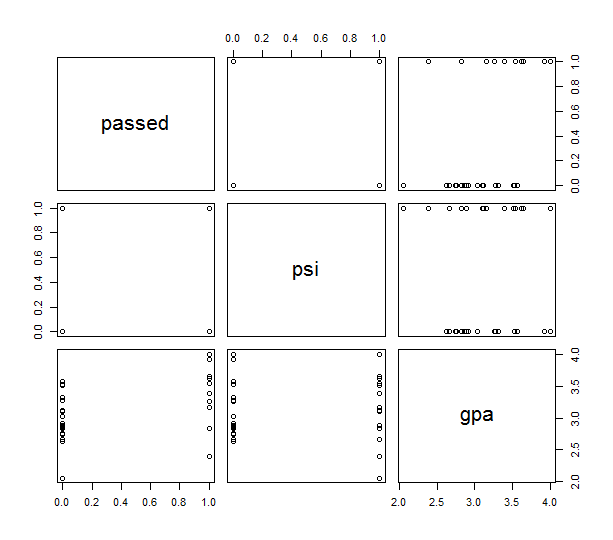
\includegraphics[scale=0.3]{../results/2_1.png}
          \caption{Scatter plots of data in psi.txt}
      \end{figure}
      
      As we can see, the nature of the data with factors, such as \textit{psi} 0 or 1, and \textit{pass} 0 or 1 make it difficult to analyse the data using scatter plots.    
    
    \subsection*{2}
    Fitting a logistic regression model with psi and gpa as explanatory variables for the outcome being that the student passed their assessment or not, we obtain the following table:
    	\begin{figure}[H]
    	\begin{lstlisting}[language=R]
	Coefficients:
            Estimate Std. Error z value Pr(>|z|)   
(Intercept)  -11.602      4.213  -2.754  0.00589 **
psi            2.338      1.041   2.246  0.02470 * 
gpa            3.063      1.223   2.505  0.01224 * 
---
Signif. codes:  
0 ‘***’ 0.001 ‘**’ 0.01 ‘*’ 0.05 ‘.’ 0.1 ‘ ’ 1
    	\end{lstlisting}
    	\caption{Parameter estimation for logistic regression model}
    	\label{fig:log_reg}
    \end{figure}
    
    Thus we determine that our logistic regression model should be:
    \begin{equation}
   	Pr(\textit{pass = 1}) = \frac{\exp(-11.602 + 2.338*\textit{psi} + 3.063*\textit{gpa})}{1 + \exp(-11.602 + 2.338*\textit{psi} + 3.063*\textit{gpa})}
    \end{equation}
    \subsection*{3}
    Based on the p-value obtained in Figure:\ref{fig:log_reg}, we reject the null hypothesis that there is no effect of psi on the outcomes of the students final assessment. Further based on our parameters for the logistic regression model, we see that a positive value, ie. 1, for \textit{psi} causes an increase in probability of passing, so we conclude that \textit{psi} does in fact work.
    \subsection*{4}
    To estimate the probability that a student with a \textit{gpa} equal to 3 who receives \textit{psi} passes the assignment, we simply enter our values into equation 1, our logistic regression model.
    \[
    Pr(\textit{pass = 1}) = \frac{\exp(-11.602 + 2.338*(1) + 3.063*(3))}{1 + \exp(-11.602 + 2.338(1) + 3.063*(3))} = 0.4813
    \]
    So there is a 48.13 \% chance of a student with \textit{gpa} of 3 who receives \textit{psi} of passing the final assignment.
    
    Similarly if we wish to estimate the probability that a student with a \textit{gpa} of 3 who does not receive \textit{psi} passing the final assignment, we simply replace the value of \textit{psi} with 0, and substitute this into equation 1
    \[
    Pr(\textit{pass = 1}) = \frac{\exp(-11.602 + 2.338*(0) + 3.063*(3))}{1 + \exp(-11.602 + 2.338(0) + 3.063*(3))} = 0.0822
    \]
    Thus there is a 8.22 \% chance of a student with a \textit{gpa} of 3 who did not take \textit{psi} passing the final assignment.
    \subsection*{5}
    We may investigate the relative change in odds of passing the final assignment for students with \textit{psi} rather than those without \textit{psi} by simply taking the exponential of the change in our linear predictor, in this case taking \textit{psi} = 1 as opposed to 0 increases our linear predictor by 2.338 as we can see in Figure:\ref{fig:log_reg}, thus our difference in odds is $exp(2.338) = 10.3605$.
    
    \subsection*{6}
    Using the alternative method of analysis, and obtaining the matrix as is outlined in the R-code section 2.6
        	\begin{figure}[H]
    	\begin{lstlisting}[language=R]
     [,1] [,2]
[1,]    3    8
[2,]   15    6
    	\end{lstlisting}
    \end{figure}
    Column [,1] represents students that did not receive \textit{psi}, where column [,2] are those students that did receive \textit{psi}. Row [1,] represents students that passed the final assignment, and row [2,] are those who did not pass. Thus 15 is the number of students that did not receive \textit{psi} and did not pass the final assignment, where 6 is the number of students that did receive \textit{psi} and also did not pass the final assignment.
    
    Performing the Fisher Test as outline in R-code section 2.6, we obtain the following:
            	\begin{figure}[H]
    	\begin{lstlisting}[language=R]
	Fisher's Exact Test for Count Data

data:x
p-value=0.0265
alternative hypothesis: true odds ratio is not equal to 1
95 percent confidence interval: 0.02016297 0.95505763
sample estimates:
odds ratio 
0.1605805 
    	\end{lstlisting}
    \end{figure}
    The conclusion is that with a p-value of 0.0265, we should reject the null hypothesis that the probability of success for students who did and did not receive \textit{psi} is equal, thus we conclude \textit{psi} does increase a students chances of passing.
    \subsection*{7}
    This second approach is not wrong.
    \subsection*{8}
	This second approach is has one main advantage, it is very simple, however it does not produce very detailed results as with the first method. The first method is more complicated, but it allows us to explore the behaviour of explanatory variables in depth.
  \section*{Exercise 3}
    \subsection*{1}
      \begin{figure}[H]
          \centering
          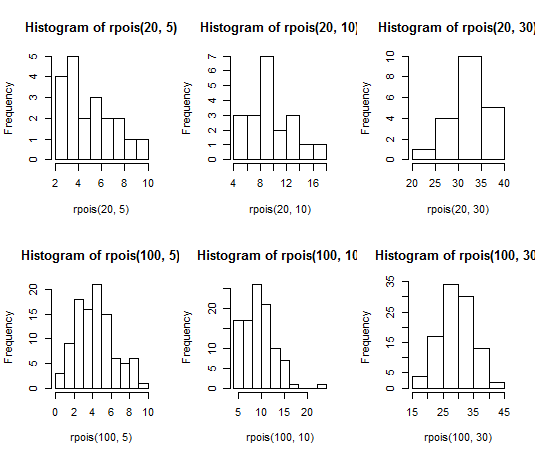
\includegraphics[scale=0.3]{../results/3_1.png}
          \caption{Histograms of random poisson with different parameters}
          \label{fig:Hist3_1}
      \end{figure}

    \subsection*{2}
      In Fig 9 different random poissons distributions are shown within the same location-scale family.
      Graphically it is easy to explain why they are in the same location-scale family.
      All the graphs seem to be more or less normally distributed,
      the only difference is that the mean and the height of the histograms are different.
      To make the mean the same, the location can be transformed and to make the height the same the scale can be transformed.
      Then you have more or less the same histograms for all the poisson distributions.
      \begin{figure}[H]
          \centering
          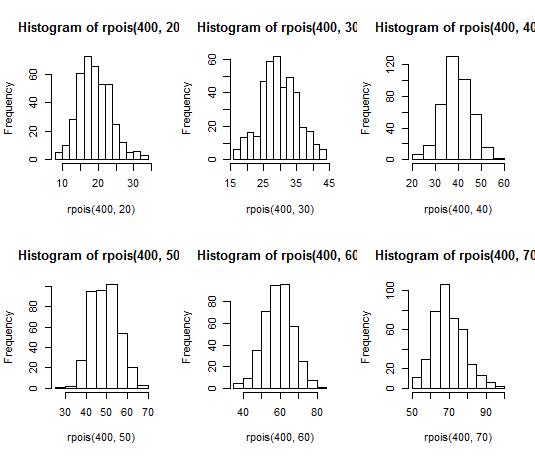
\includegraphics[scale=0.3]{../results/3_2.png}
          \caption{Histograms of random poisson with different parameters, within the same location-scale family}
          \label{fig:Hist3_2}
      \end{figure}

    \subsection*{3}
    From our summary:
        \begin{lstlisting}[language=R]
Coefficients:
              Estimate Std. Error z value Pr(>|z|)   
(Intercept) -0.5102693  0.9053301  -0.564  0.57301   
oligarchy    0.0730814  0.0345958   2.112  0.03465 * 
pollib      -0.7129779  0.2725635  -2.616  0.00890 **
parties      0.0307739  0.0111873   2.751  0.00595 **
pctvote      0.0138722  0.0097526   1.422  0.15491   
popn         0.0093429  0.0065950   1.417  0.15658   
size        -0.0001900  0.0002485  -0.765  0.44447   
numelec     -0.0160783  0.0654842  -0.246  0.80605   
numregim     0.1917349  0.2292890   0.836  0.40303 
      \end{lstlisting}
      We are able to obtain a linear model that will allow us to estimate longevity for various conditions, thus our model is:
      \[
      miltcoup = -0.51 + 0.07*oligarchy - 0.71 * pollib + 0.03 * parties + 0.01 * pctvote + 0.01 * popn -0.0001 * size -0.02 * numelec + 0.19 * numregim
      \]

    \subsection*{4}
      With the step-down method we remove at each step the feature with the highest p-value.
      In this model the steps are as follows:
      \begin{itemize}
        \item miltcoup ~ oligarchy + pollib + parties + pctvote + popn + size + numregim + numelec\\ The highest p-value is numelec
        \item miltcoup ~ oligarchy + pollib + parties + pctvote + popn + size + numregim\\ The highest p-value is numregim
        \item miltcoup ~ oligarchy + pollib + parties + pctvote + popn + size\\ The highest p-value is size
        \item miltcoup ~ oligarchy + pollib + parties + pctvote + popn\\ The highest p-value is popn
        \item miltcoup ~ oligarchy + pollib + parties + pctvote\\ The highest p-value is pctvote
        \item miltcoup ~ oligarchy + pollib + parties\\ Stop here
      \end{itemize}

    \subsection*{5}
      The plots found in Fig\ref{fig:3_5} are a bit strange, but because both methods show the same behaviour, the weird shapes are not a result of us taking out too many variables
      We do not know the reason why they show this behaviour.

      \begin{figure}[H]
          \centering
          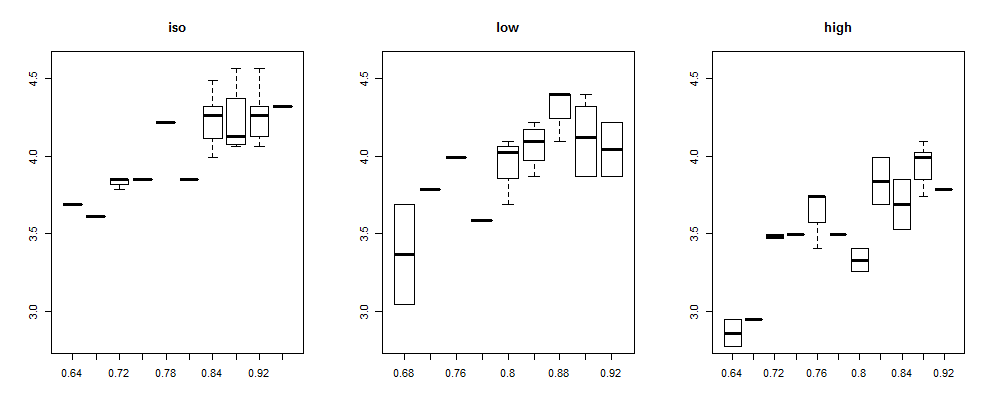
\includegraphics[scale=0.3]{../results/diffThoraxActivity.png}
          \caption{Plots of the reduced model (top row) and full model (bottom row)}
          \label{fig:3_5}
      \end{figure}
    
  \section{R-Code}
    \subsection{Exercise 1}\label{sec:RE1}
      \begin{lstlisting}[language=R]
      data = read.table("fruitflies.txt", header=T)
attach(data)

#1.1
#loading data
data$loglongevity = log(longevity)
attach(data)

#1.2
#Various plots
par(mfrow=c(1,2))
plot(activity, loglongevity)
plot(thorax, loglongevity); abline(thorax, loglongevity)
par(mfrow=c(1,1))
pairs(data)


#1.3
activitylm = lm(loglongevity~activity,data=data)
# we reject H0 so the activity has an influence on the longevity
anova(activitylm)

#1.4
#box plots of log(longevity) and activity
boxplot(loglongevity~activity)
iso = data[activity=="isolated", ]
low = data[activity=="low", ]
high = data[activity=="high", ]
summary(iso)
summary(low)
summary(high)
summary(activitylm)

#1.5
activityThoraxlm = lm(loglongevity~activity+thorax,data=data)
# we reject H0 so the activity and thorax has an influence on the longevity
anova(activityThoraxlm)

#1.6
summary(activityThoraxlm)
mean(data$thorax)
#high
mean(data$thorax)*2.97899+1.21893
#isolated
mean(data$thorax)*2.97899+1.21893+0.40998
#low
mean(data$thorax)*2.97899+1.21893+0.28570

min(data$thorax)
#high
min(data$thorax)*2.97899+1.21893
#isolated
min(data$thorax)*2.97899+1.21893+0.40998
#low
min(data$thorax)*2.97899+1.21893+0.28570

#1.7
plot(thorax,loglongevity, xlab="thorax length",ylab="log(longevity)")
par(mfrow = c(1,3))
boxplot(loglongevity ~ thorax, data=iso, ylim = c(2.8, 4.6), main="iso")
boxplot(loglongevity ~ thorax, data=low, ylim = c(2.8, 4.6), main="low")
boxplot(loglongevity ~ thorax, data=high, ylim = c(2.8, 4.6), main="high")

#1.9
par(mfrow = c(1,2))
qqnorm(residuals(activityThoraxlm))
plot(fitted(activityThoraxlm), residuals(activityThoraxlm))

#1.10
longevitylm = lm(longevity~activity+thorax)
anova(longevitylm)
par(mfrow = c(1,2))
qqnorm(residuals(longevitylm))
plot(fitted(longevitylm), residuals(longevitylm))

      \end{lstlisting}
    \subsection{Exercise 2}\label{sec:RE2}
      \begin{lstlisting}[language=R]
      #2.1
data = read.table("psi.txt", header=T)
attach(data)

#Table and histogram
tot=xtabs(~psi+passed); tot
pairs(data)

#2.2

#Estimation
passedlm = glm(passed~psi+gpa,family=binomial)
summary(passedlm)

data$psi=factor(data$psi)
data$gpa=factor(data$gpa)
passedlm2 = glm(passed~psi+gpa, family=binomial)
summary(passedlm2)

plot(c(0,coef(passedlm2)[2:3]),type="l")

#2.3
#Addording to p-values, psi works

#2.4

#function to predict passing, x=psi, y=gpa
passest <- function(x,y) {exp(-11.602 + 2.338*x + 3.063*y)/(1 + exp(-11.602 + 2.338*x + 3.063*y))}

#student with gpa 3 and received psi
passest(1,3)
#student with gpa 3 and did not receive psi
passest(0,3)

#2.5
#Increase in odds from having psi vs not having psi
passodds <- function(p,q) {exp(-11.602 + 2.338*p + 3.063*q)}

#2.6
x=matrix(c(3,15,8,6),2,2);x
#if we look at tot, we can see 15 represents students that
#did not receive psi, and did not pass
#6 are those students who did receive psi, but still did not pass
fisher.test(x)

#test concludes that the effects of psi and pass are not
#independant

#2.7

      \end{lstlisting}
    \subsection{Exercise 3}\label{sec:RE3}
      \begin{lstlisting}[language=R]
      data = read.table("africa.txt", header=T)
attach(data)

#3.1
par(mfrow=c(2,3))
hist(rpois(20,5))
hist(rpois(20,10))
hist(rpois(20,30))
hist(rpois(100,5))
hist(rpois(100,10))
hist(rpois(100,30))

hist(rpois(300,10))
hist(rpois(300,20))
hist(rpois(300,30))
hist(rpois(400,10))
hist(rpois(400,20))
hist(rpois(400,30))

#3.2
hist(rpois(400,20))
hist(rpois(400,30))
hist(rpois(400,40))
hist(rpois(400,50))
hist(rpois(400,60))
hist(rpois(400,70))
par(mfrow=c(1,1))

#3.3

fullafricalm = glm(miltcoup~oligarchy+pollib+parties+pctvote
               +popn+size+numelec+numregim, family=poisson,data=data)
summary(fullafricalm)

#3.4
#remove numelec, has highest p-value

africalm = glm(miltcoup~oligarchy+pollib+parties+pctvote
               +popn+size+numregim, family=poisson,data=data)
summary(africalm)

#remove numregim, has highest p-value

africalm = glm(miltcoup~oligarchy+pollib+parties+pctvote
               +popn+size, family=poisson,data=data)
summary(africalm)

#remove size, has highest p-value

africalm = glm(miltcoup~oligarchy+pollib+parties+pctvote
               +popn, family=poisson,data=data)
summary(africalm)

#remove popn, has highest p-value

africalm = glm(miltcoup~oligarchy+pollib+parties+pctvote,
               family=poisson,data=data)
summary(africalm)

#remove pctvote, has highest p-value

africalm = glm(miltcoup~oligarchy+pollib+parties,
               family=poisson,data=data)
summary(africalm)

confint(africalm)
coef(africalm)

#3.5

#plot of model
plot(fitted(africalm),residuals(africalm))
plot(log(fitted(africalm)),residuals(africalm))
plot(log(fitted(africalm)),residuals(africalm,type="response"))
#plots of full model
plot(fitted(fullafricalm),residuals(fullafricalm))
plot(log(fitted(fullafricalm)),residuals(fullafricalm))
plot(log(fitted(fullafricalm)),residuals(fullafricalm,type="response"))

pairs(miltcoup~oligarchy+pollib+parties,data=data)

data$pollib = as.factor(data$pollib)
africalm = glm(miltcoup~oligarchy+pollib+parties,
               family=poisson,data=data)
summary(africalm)

pairs(miltcoup~oligarchy+parties,data=data)
      \end{lstlisting}
\end{document}
